\begin{frame}
\titlepage
\end{frame}

\begin{frame}
\frametitle{Overview}
\tableofcontents
\end{frame}



\section{Introduction}

	\begin{frame}
	\frametitle{Why Disentangle Causal Factors?}
		\begin{figure}[htp]
			\centering
			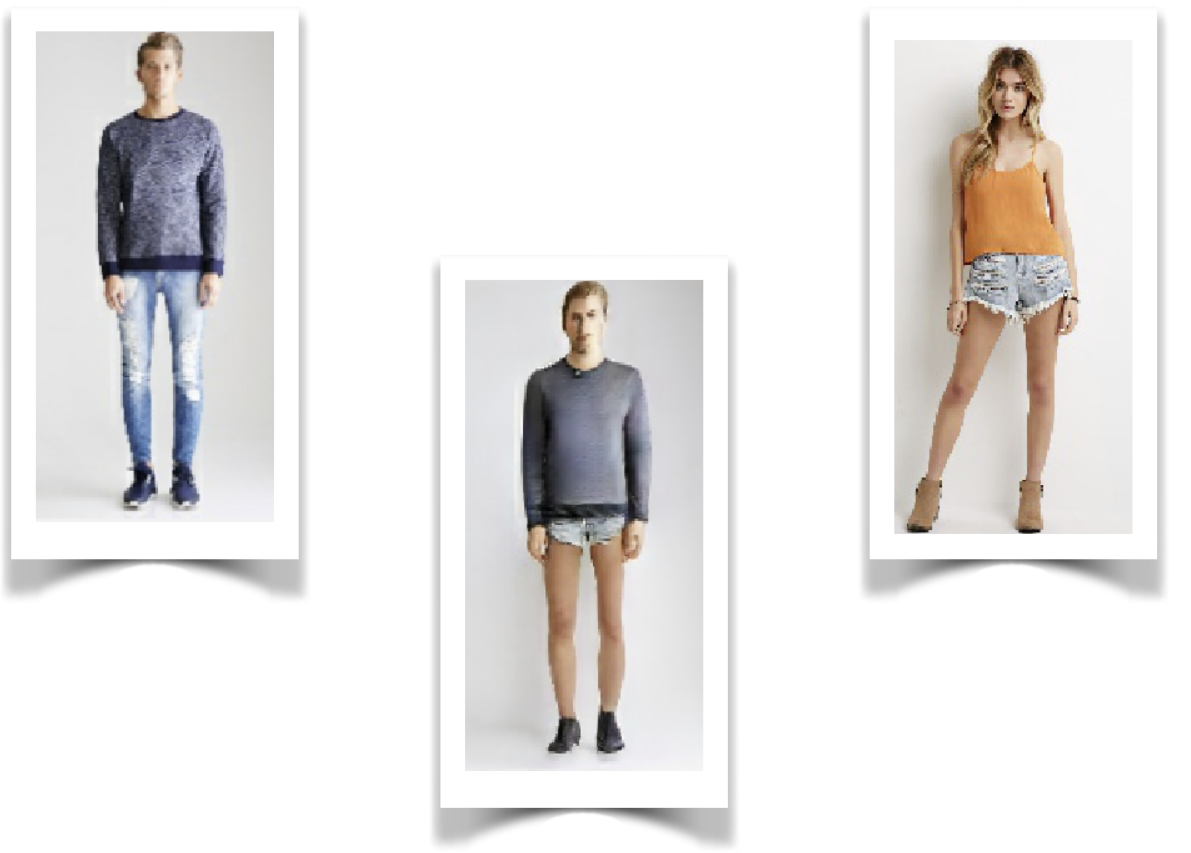
\includegraphics[trim={0cm 0cm 0cm 0cm},clip, width=0.4\linewidth]{fig/other/hotpants}
			\caption{\textit{"Imagine, how ridiculous you would look if you wore that hot pants"} - Thought experiments are a targeted manipulation of a disentangled representation.}
			\label{fig:hotpants}
		\end{figure}
	\end{frame}

	\begin{frame}
	\frametitle{How Not to Disentangle.}
		\begin{figure}[htp]
			\centering
			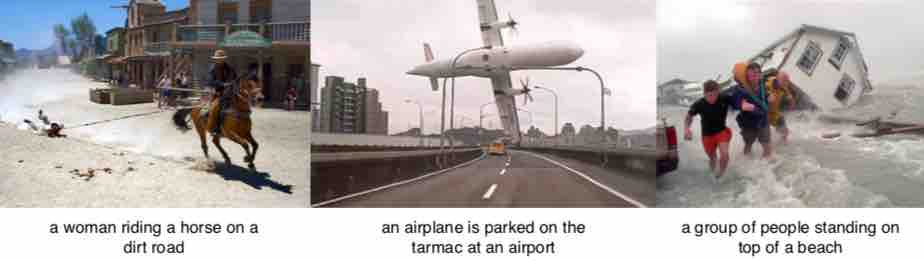
\includegraphics[trim={0cm 0cm 0cm 0cm},clip, width=1.\linewidth]{fig/other/notcausal}
			\caption{The image captions are generated by a deep neural network (Neuraltalk2) \cite{karpathy15neuraltalk}. Yet, common sense understanding of psychological and physical entities in terms of causal relationships and narratives is absent \cite{tenenbaum18think}. Instead, the neural network seems to capture mere associations.}
			\label{fig:notcausal}
		\end{figure}
	\end{frame}

	\begin{frame}
	\frametitle{How can Humans Disentangle?}
		\begin{itemize}
			\item Priors:
			\item Data: temporal and interventional
			\note{image of child which destroys something}
			\item Models
		\end{itemize}
	\end{frame}

	\begin{frame}
	\frametitle{Contributions}
		\begin{itemize}
			\item  \textit{Hypothesis \emph{i)}: Unsupervised learning of object shape benefits from abstracting away the complement of shape, namely the object appearance. Explaining away the appearance factor can be achieved by a disentangled generative modelling of both factors.}
			\item \textit{Hypothesis \emph{ii)}: Learning unsupervised disentanglement without any assumptions is fundamentally impossible. In accordance with the literature on causal learning \cite{pearl18impediments}, disentangling causal factors requires model assumptions and/or interactional data - instead of observational (raw) data.}
		\end{itemize}
	\end{frame}



\section{Prerequisites}
	\subsection{Learning from Data}
	\subsection{Disentangling}
	\subsection{Causality}

\section{Method}
	\begin{frame}
	\frametitle{Disentangling by Transforming}
		\begin{figure}[t]
			\centering
			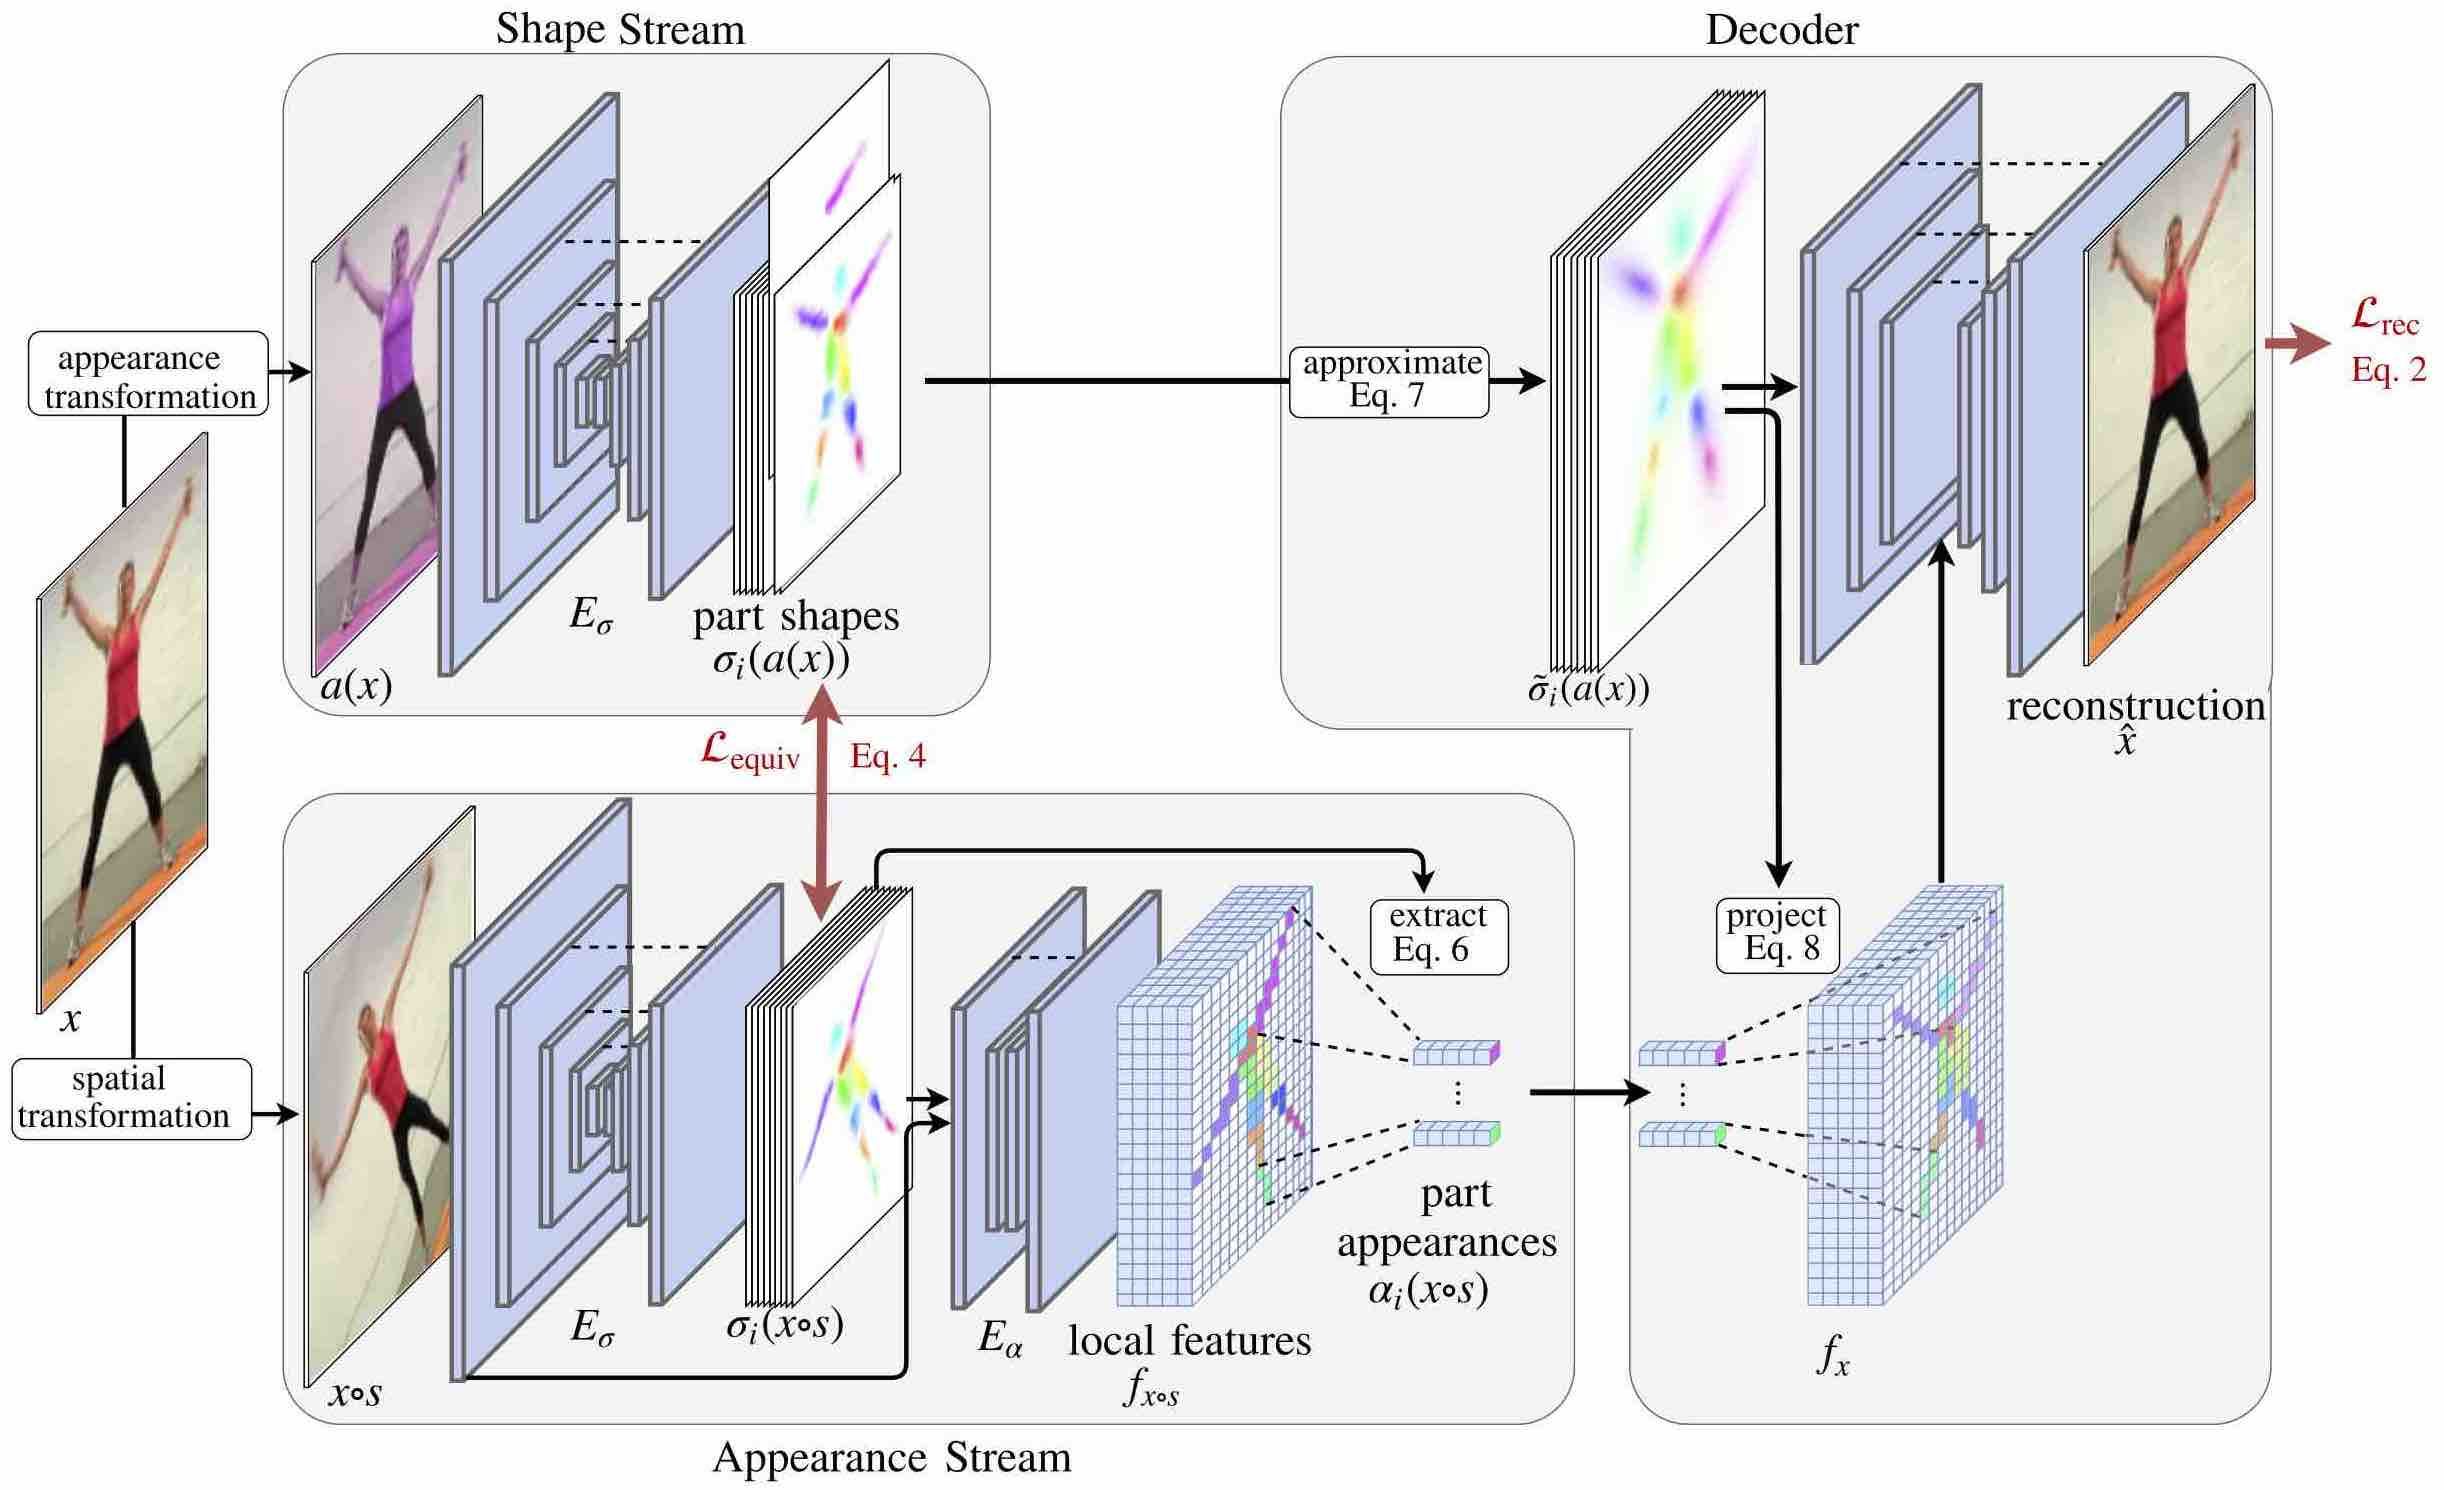
\includegraphics[trim={0cm 0cm 0cm 0cm},clip, width=1.\linewidth]{fig/other/architecture_final}
			\caption{Encoder $E$ encodes shape and appearance for two transformed images $s(\mathbf{x})$ and $a(\mathbf{x})$, after recombination $R$ of $({\alpha}_{s(\mathbf{x})}, {\sigma}_{a(\mathbf{x})})$ into latent image $Z$, the decoder $D$ reconstructs the image $\mathbf{x}$.}
			\label{fig:architecture}
		\end{figure}
	\end{frame}

	\begin{frame}
	\frametitle{Invariance and Equivariance}
		\begin{align}
			{\alpha}_{s(\mathbf{x})}  &= {\alpha}_{\mathbf{x}} \tag{invariance of appearance}\\
			{\sigma}_{a(\mathbf{x})} &= {\sigma}_{\mathbf{x}}  \tag{invariance of shape}\\
			{\sigma}_{s(\mathbf{x})} &= s({\sigma}_{\mathbf{x}}) \tag{equivariance of shape}
		\label{eq:invar}
		\end{align} % quad \forall i \leq n
	\end{frame}

	\begin{frame}
	\frametitle{Objective}
		\begin{equation}\label{eq:loss_rec}
			\mathcal{L}_{\textrm{rec}}= \lVert  \mathbf{x}  - \mathrm{D}[{\alpha}_{s(\mathbf{x})}, {\sigma}_{a(\mathbf{x})}]\rVert
		\end{equation}

		\begin{equation}
			\mathcal{l}_{\textrm{equiv}}^i = \mathcal{l}_{\mu}^i+ \mathcal{l}_{\sigma}^i
		\label{covariance}
		\end{equation}
		The overall loss objective is the sum of the reconstruction loss and the equivariance loss for all $n$ parts:
		\begin{equation}
		\mathcal{L} = \sum_{i=1}^n \mathcal{L}_{\text{equiv}}^i + \mathcal{L}_{\textrm{rec}}
		\end{equation}
	\end{frame}




\section{Object Shape Learning}
	\begin{frame}
	\frametitle{Learned Shapes}
		% PENN SHAPES
		\begin{figure}[htp]
			\begin{subfigure}{1.\textwidth}
			\centering
			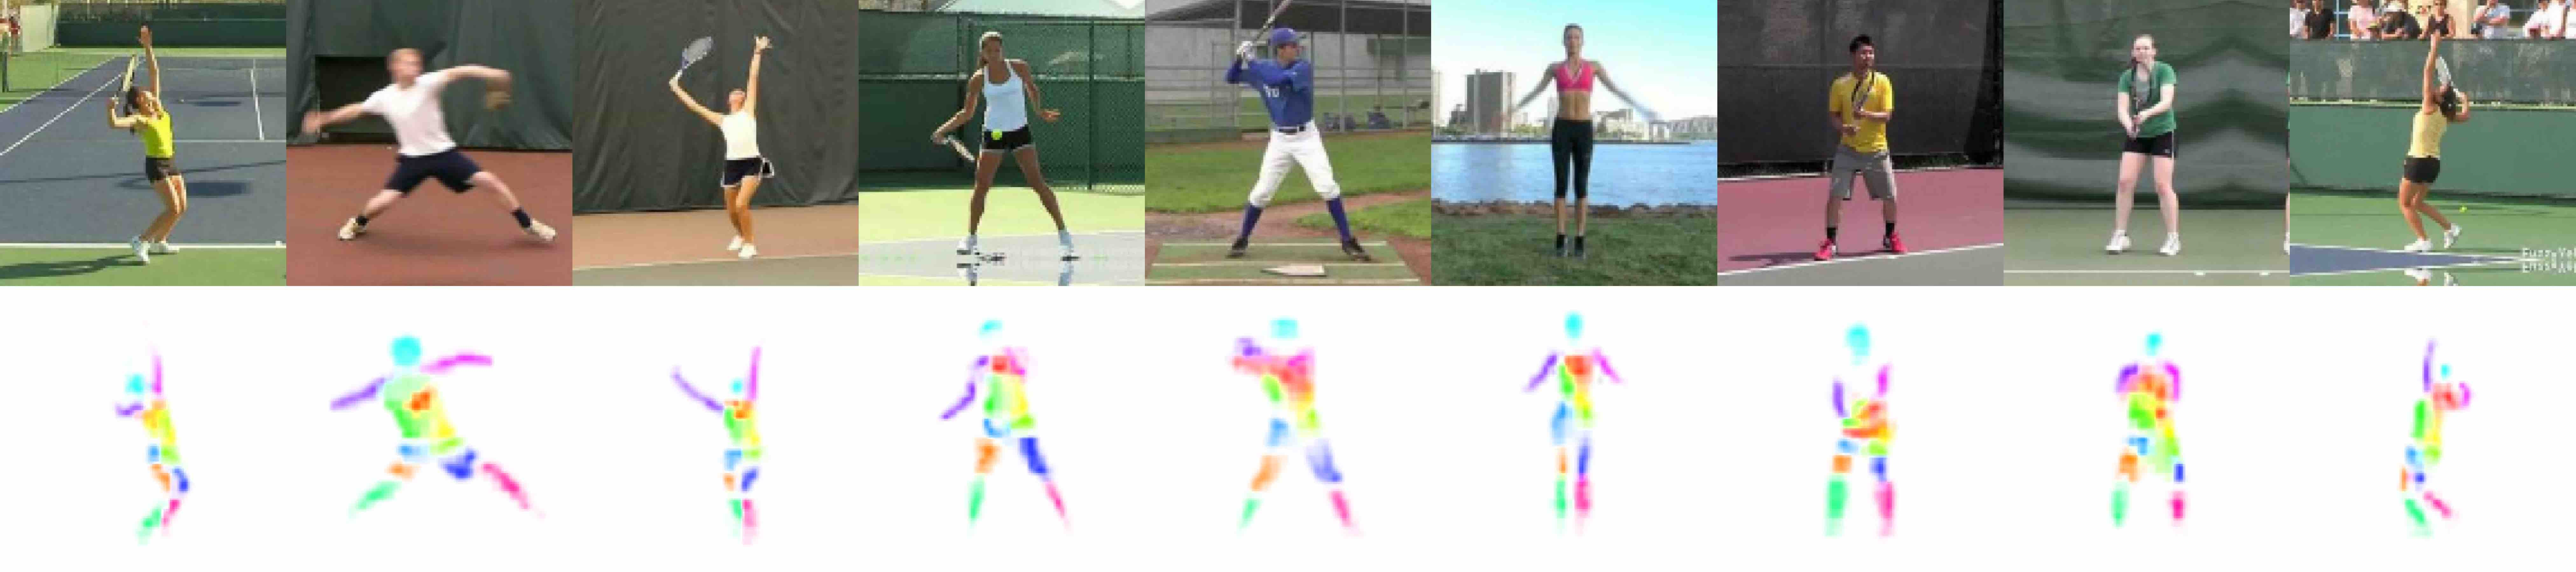
\includegraphics[trim={0cm 0cm 0cm 0cm},clip, width=1.\linewidth]{fig/shape/shape8white}\caption{}
			\label{fig:shape_penn}
			\end{subfigure}
			\begin{subfigure}{1.\textwidth}
			\centering
			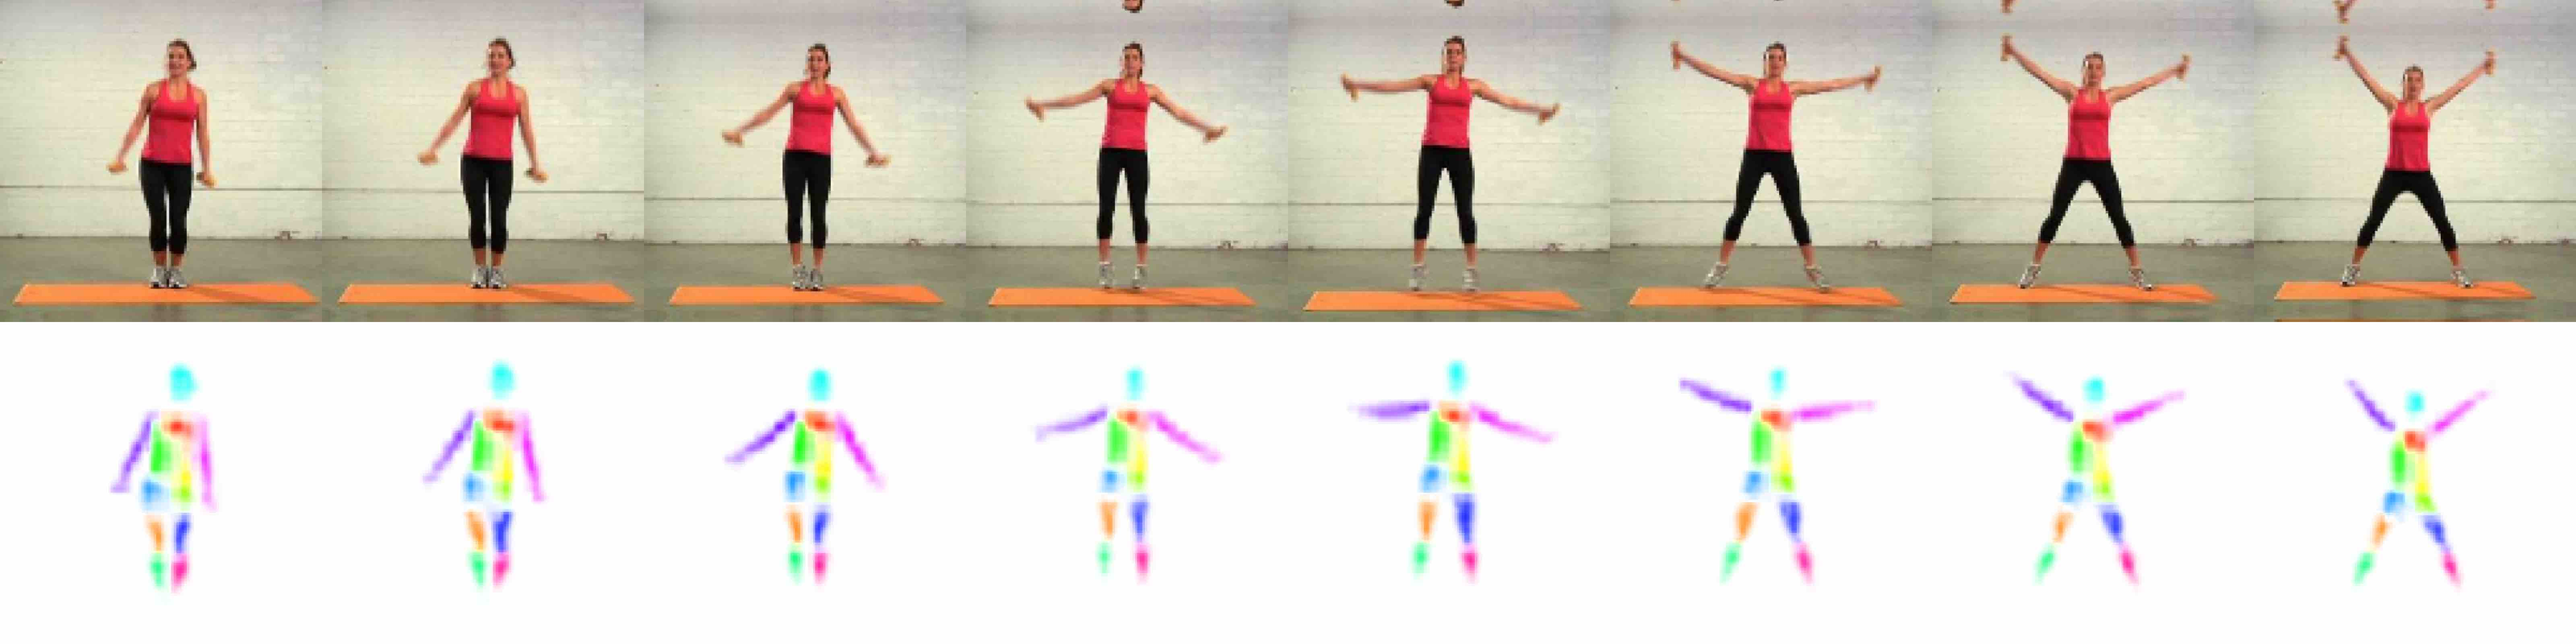
\includegraphics[trim={0cm 0cm 0cm 0cm},clip, width=1.\linewidth]{fig//shape/shape_yoga8}\caption{}
			\label{fig:shape_tennis}
			\end{subfigure}
			\caption{Learned shape representation on Penn Action. For visualization, 13 of 16 part activation maps are plotted in one image. (a) Different instances, showing intra-class consistency and (b) video sequence, showing consistency and smoothness under motion, although each frame is processed individually.}
			\label{fig:shape}
		\end{figure}
	\end{frame}

	\begin{frame}
	\frametitle{Landmark Regression}
		\begin{itemize}
			\item Protocol from Thewlis
		\end{itemize}
	\end{frame}

	\begin{frame}
	\frametitle{Human and Cat Faces}
		% FACES
		\begin{figure}[htp]
			\centering
			\begin{subfigure}{1.\textwidth}
			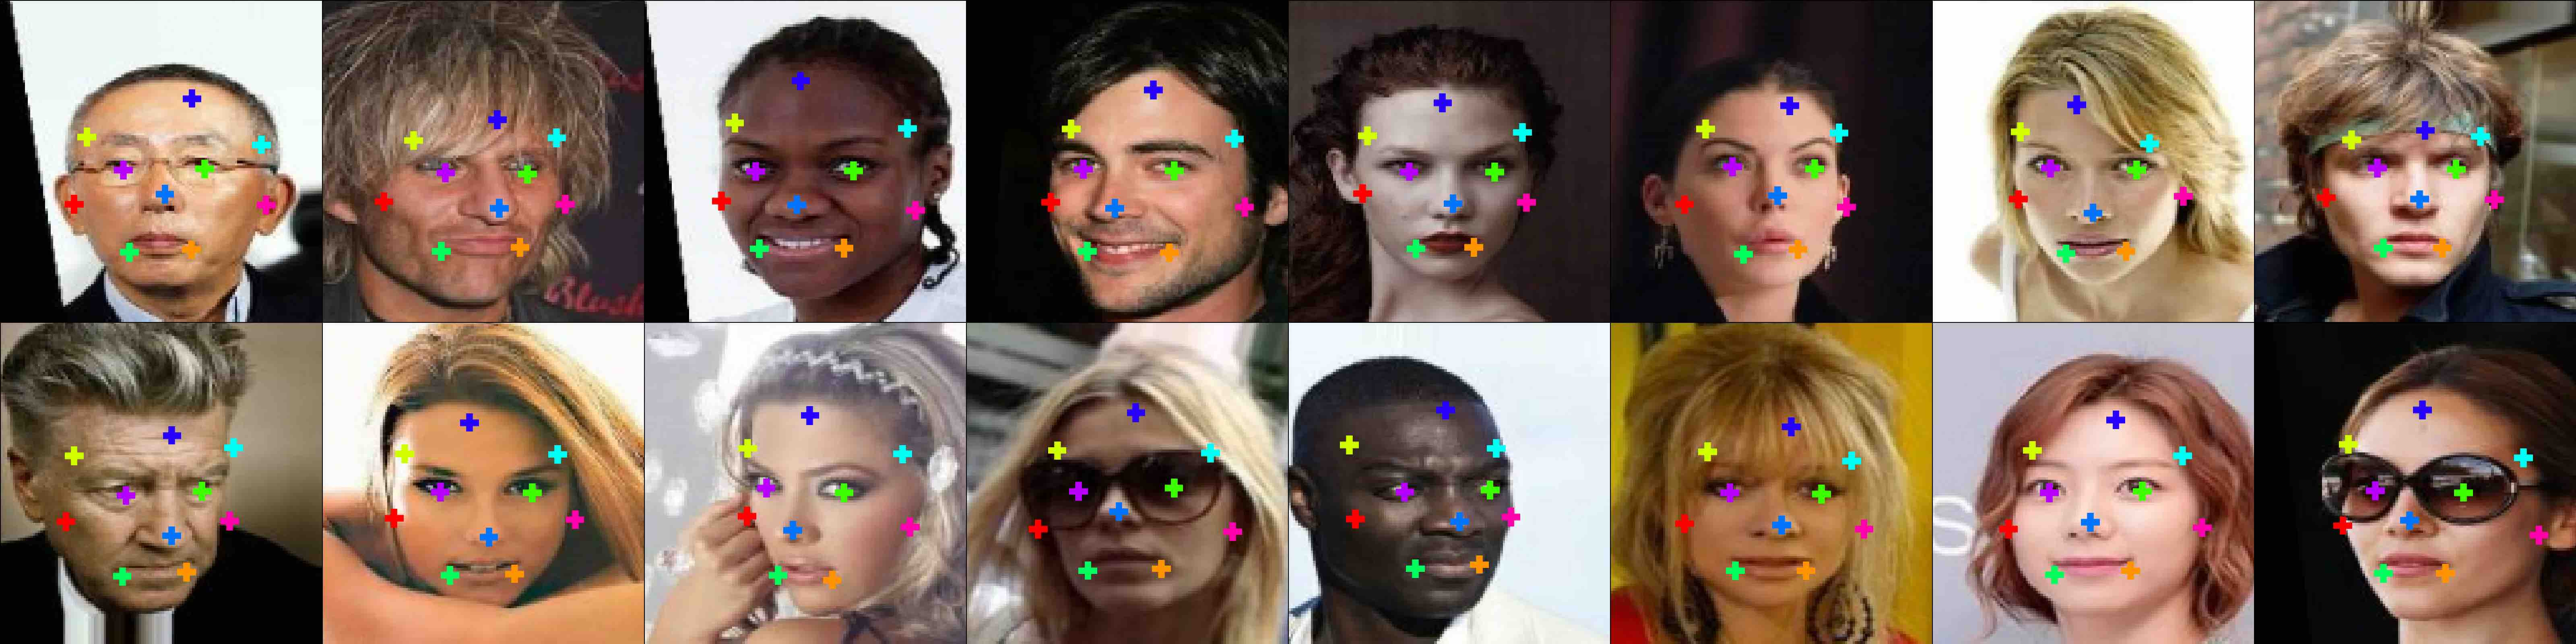
\includegraphics[trim={0cm 0cm 0cm 0cm},clip, width=1.\linewidth]{fig/shape/0celeba}\caption{}
			\end{subfigure}
			\begin{subfigure}{1.\textwidth}
			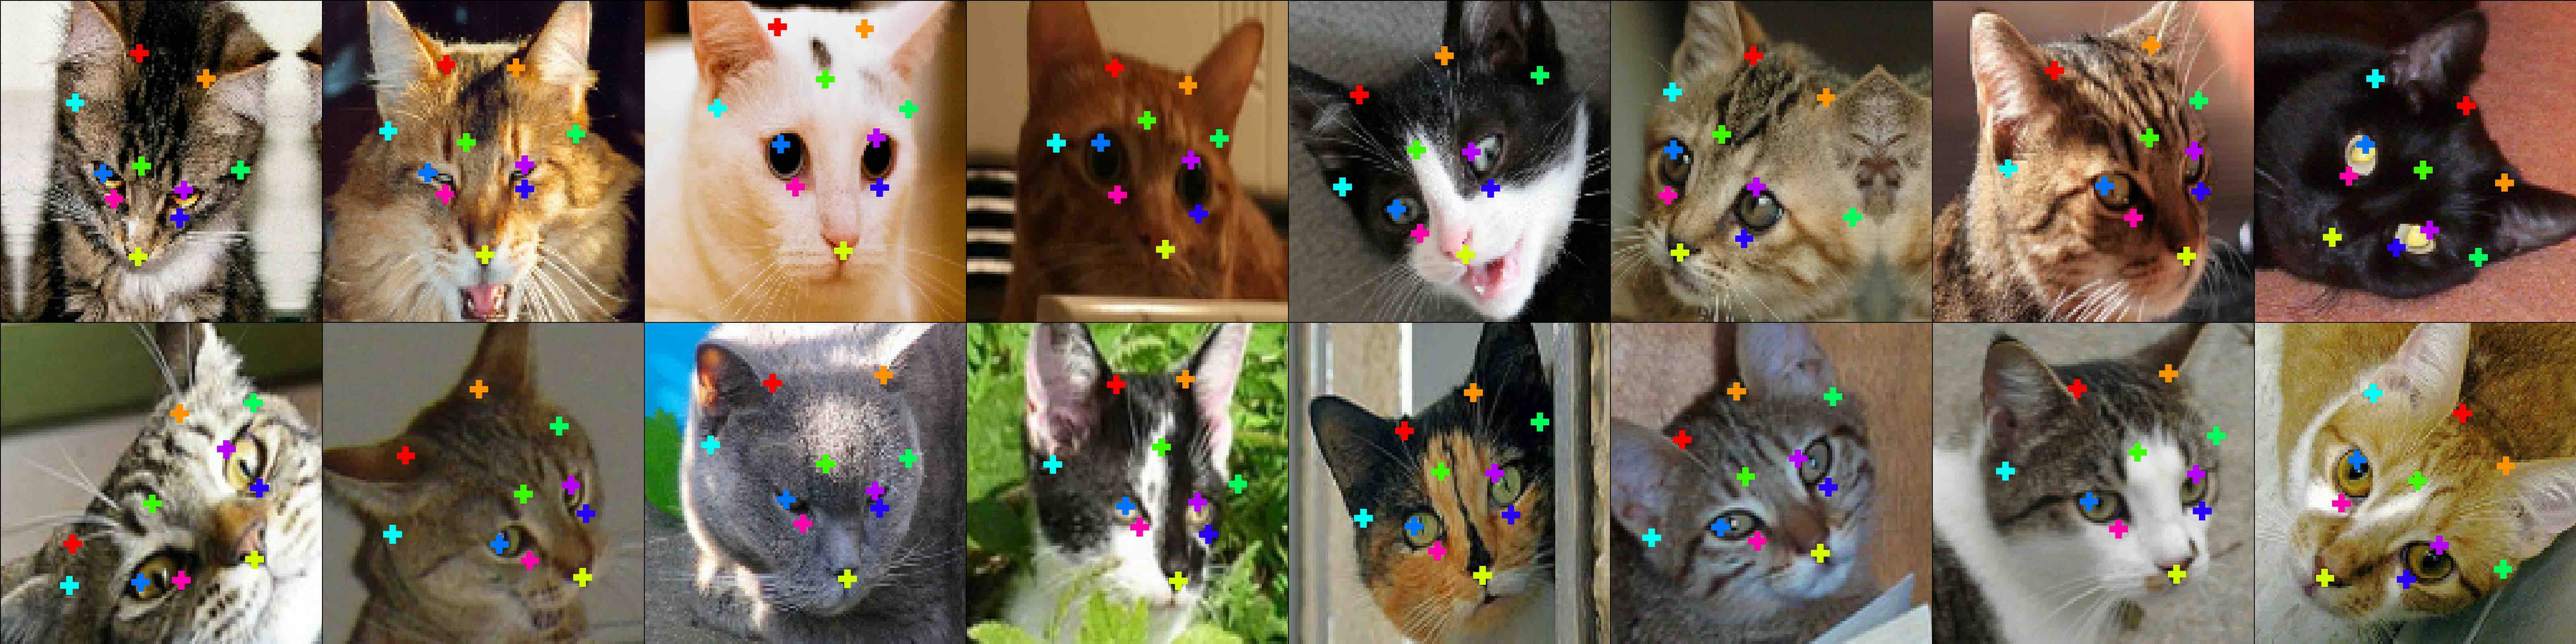
\includegraphics[trim={0cm 0cm 0cm 0cm},clip, width=1.\linewidth]{fig/shape/0cats}\caption{}
			\end{subfigure}
			\caption{{Unsupervised discovery of landmarks the object classes of (a) human (CelebA dataset) and (b) cat faces (Cat Head dataset).}}
			\label{fig:kp_faces}
		\end{figure}
	\end{frame}

	\begin{frame}
	\frametitle{Human and Cat Faces}
		\begin{table}[t]
				\caption{Error of unsupervised methods for landmark prediction on the Cat Head, MAFL (subset of CelebA) testing sets. The error is in \% of inter-ocular distance.}
				\label{tab:faces}
				\centering
				\begin{tabular}{l|ccc}
				\hline
				Dataset & Cat Head &  & MAFL \\
				  \# Landmarks &10 & 20  & 10  \\
				  \hline
				 Thewlis \cite{thewlis17}
				 & 26.76 & 26.94 & 6.32    \\
				 Jakab \cite{jakab18}
				 & - & - & 4.69  \\
				 Zhang \cite{zhang18}
				 & 15.35 & 14.84 & 3.46  \\
				  Ours & \textbf{9.88}  & \textbf{9.30} & \textbf{3.24}  \\ \hline  % image length is 600: 32.15 , 23.51
				\end{tabular}
		\end{table}
	\end{frame}






\section{Disentangling of Shape and Appearance}



